\documentclass[12pt,a4paper]{report}
\usepackage[utf8]{inputenc}
\usepackage{hyperref}
\usepackage{geometry}
\usepackage{graphicx}
\geometry{a4paper, margin=1in}

\title{lorem ipsum \\ \large MIRPR Stable Diffusion Project}
\author{Eduard-Mitrut Rosca, Albert Regus}

\begin{document}

\maketitle

\chapter*{Demo APP Functionalities \& Features}

\section*{Overview}
The application is a website featuring a canvas (similar to the one provided by \href{https://www.nvidia.com/en-us/studio/canvas/}{NVIDIA Canvas}), where users can paint simple images. The output is a realistic image generated based on the user’s preferences using a Stable Diffusion-based model.

\section*{Functionalities}
\begin{itemize}
    \item Paint on a blank canvas using different brush colors and sizes.
    \item Erase unwanted elements from the canvas.
    \item Display the generated realistic image output to the user.
\end{itemize}

\section*{Short Description}
The system leverages a Stable Diffusion-based model, such as ControlNet, to generate realistic synthetic images. This approach aims to improve the performance of AI models that require large datasets to achieve optimal results by providing an efficient way to generate training data.

\chapter*{Useful Work and Related Work}

\section*{ControlNet}
Pretrained diffusion models used for image generation.
\begin{itemize}
    \item \href{https://github.com/lllyasviel/ControlNet}{https://github.com/lllyasviel/ControlNet}
    \item \href{https://arxiv.org/pdf/2302.05543}{https://arxiv.org/pdf/2302.05543}
\end{itemize}

\section*{UNet (Used for Segmentation)}
\begin{itemize}
    \item \href{https://arxiv.org/pdf/1505.04597}{https://arxiv.org/pdf/1505.04597}
\end{itemize}

\section*{Fréchet Inception Distance (For Metrics)}
\begin{itemize}
    \item \href{https://arxiv.org/pdf/1706.08500}{https://arxiv.org/pdf/1706.08500}
\end{itemize}

\section*{Datasets}
\begin{itemize}
    \item \href{https://cs.nyu.edu/~fergus/datasets/nyu_depth_v2.html}{NYU Depth Dataset V2}
    \item \href{https://cs.nyu.edu/~fergus/datasets/indoor_seg_support.pdf}{Indoor Segmentation Support (ADE20K)}
\end{itemize}

\section*{Generative Models (StabilityAI)}
\begin{itemize}
    \item \href{https://github.com/stability-ai/generative-models}{https://github.com/stability-ai/generative-models}
\end{itemize}

\section*{Stable Diffusion}
\begin{itemize}
    \item \href{https://arxiv.org/pdf/2112.10752}{https://arxiv.org/pdf/2112.10752}
\end{itemize}


\chapter*{Training on ToyDataset}

\section*{ControlNet}
ControlNet is a pretrained diffusion model used in image generation tasks, particularly for applications that require precise control over generated outputs based on user inputs. By using control structures like edge maps or human pose estimations, ControlNet allows users to guide the diffusion process for targeted and customizable image synthesis. This feature makes it highly suitable for real-world applications where the image content needs to closely match specified criteria, making it particularly useful in tools that require user-driven adjustments to generated images.
\begin{itemize}
    \item \href{https://github.com/lllyasviel/ControlNet}{ControlNet GitHub Repository}
    \item \href{https://arxiv.org/pdf/2302.05543}{ControlNet Research Paper}
\end{itemize}

\subsection*{Fill50k DataSet}

The Fill50k dataset used in this project is specifically designed to support training in image generation tasks involving circular shapes.

- Source Images with Circle Masks: The dataset contains source images that include masks of circles. These masks serve as structural guides for models, helping them learn the spatial arrangement and shape of circles within an image. By providing masked regions, these source images establish the foundational patterns that guide the model in generating circular forms.

- Target Images for Training: In addition to source images with masks, Fill50k includes target images, which are the desired outputs the model aims to replicate or generate. These target images allow the model to learn the texture, color, and lighting details that should fill the circular masked areas, effectively helping it understand how to realistically render circles.

- Text Prompts: Each image in the Fill50k dataset is associated with a specific prompt used during training. These prompts describe the image content, helping the model learn to associate textual descriptions with visual features.

\subsection*{How We Used ControlNet}
In our project, we trained the ControlNet model to generate circular images by training it for 3 and 5 epochs on a dataset of 512 images from the Fill50k dataset. This customization allows the model to produce outputs tailored to our specific requirements for generating circle images on the application’s canvas.

We used the Stable Diffusion 2.1 (SD2.1) model for training. However, since the training was performed on a limited dataset of only 512 images, we encountered some inconsistencies in the generated images. Specifically, although the model was trained to generate circular images based on a prompt, the textures in the background of the generated images did not always match those found in the training data (example: Figure2). This issue arose because the limited size and diversity of the training dataset resulted in insufficient generalization of background textures for the same prompts. Despite this, the model was able to capture the core features, such as shapes and structures, while the textures varied depending on the context of the input.

\begin{figure}
    \centering
    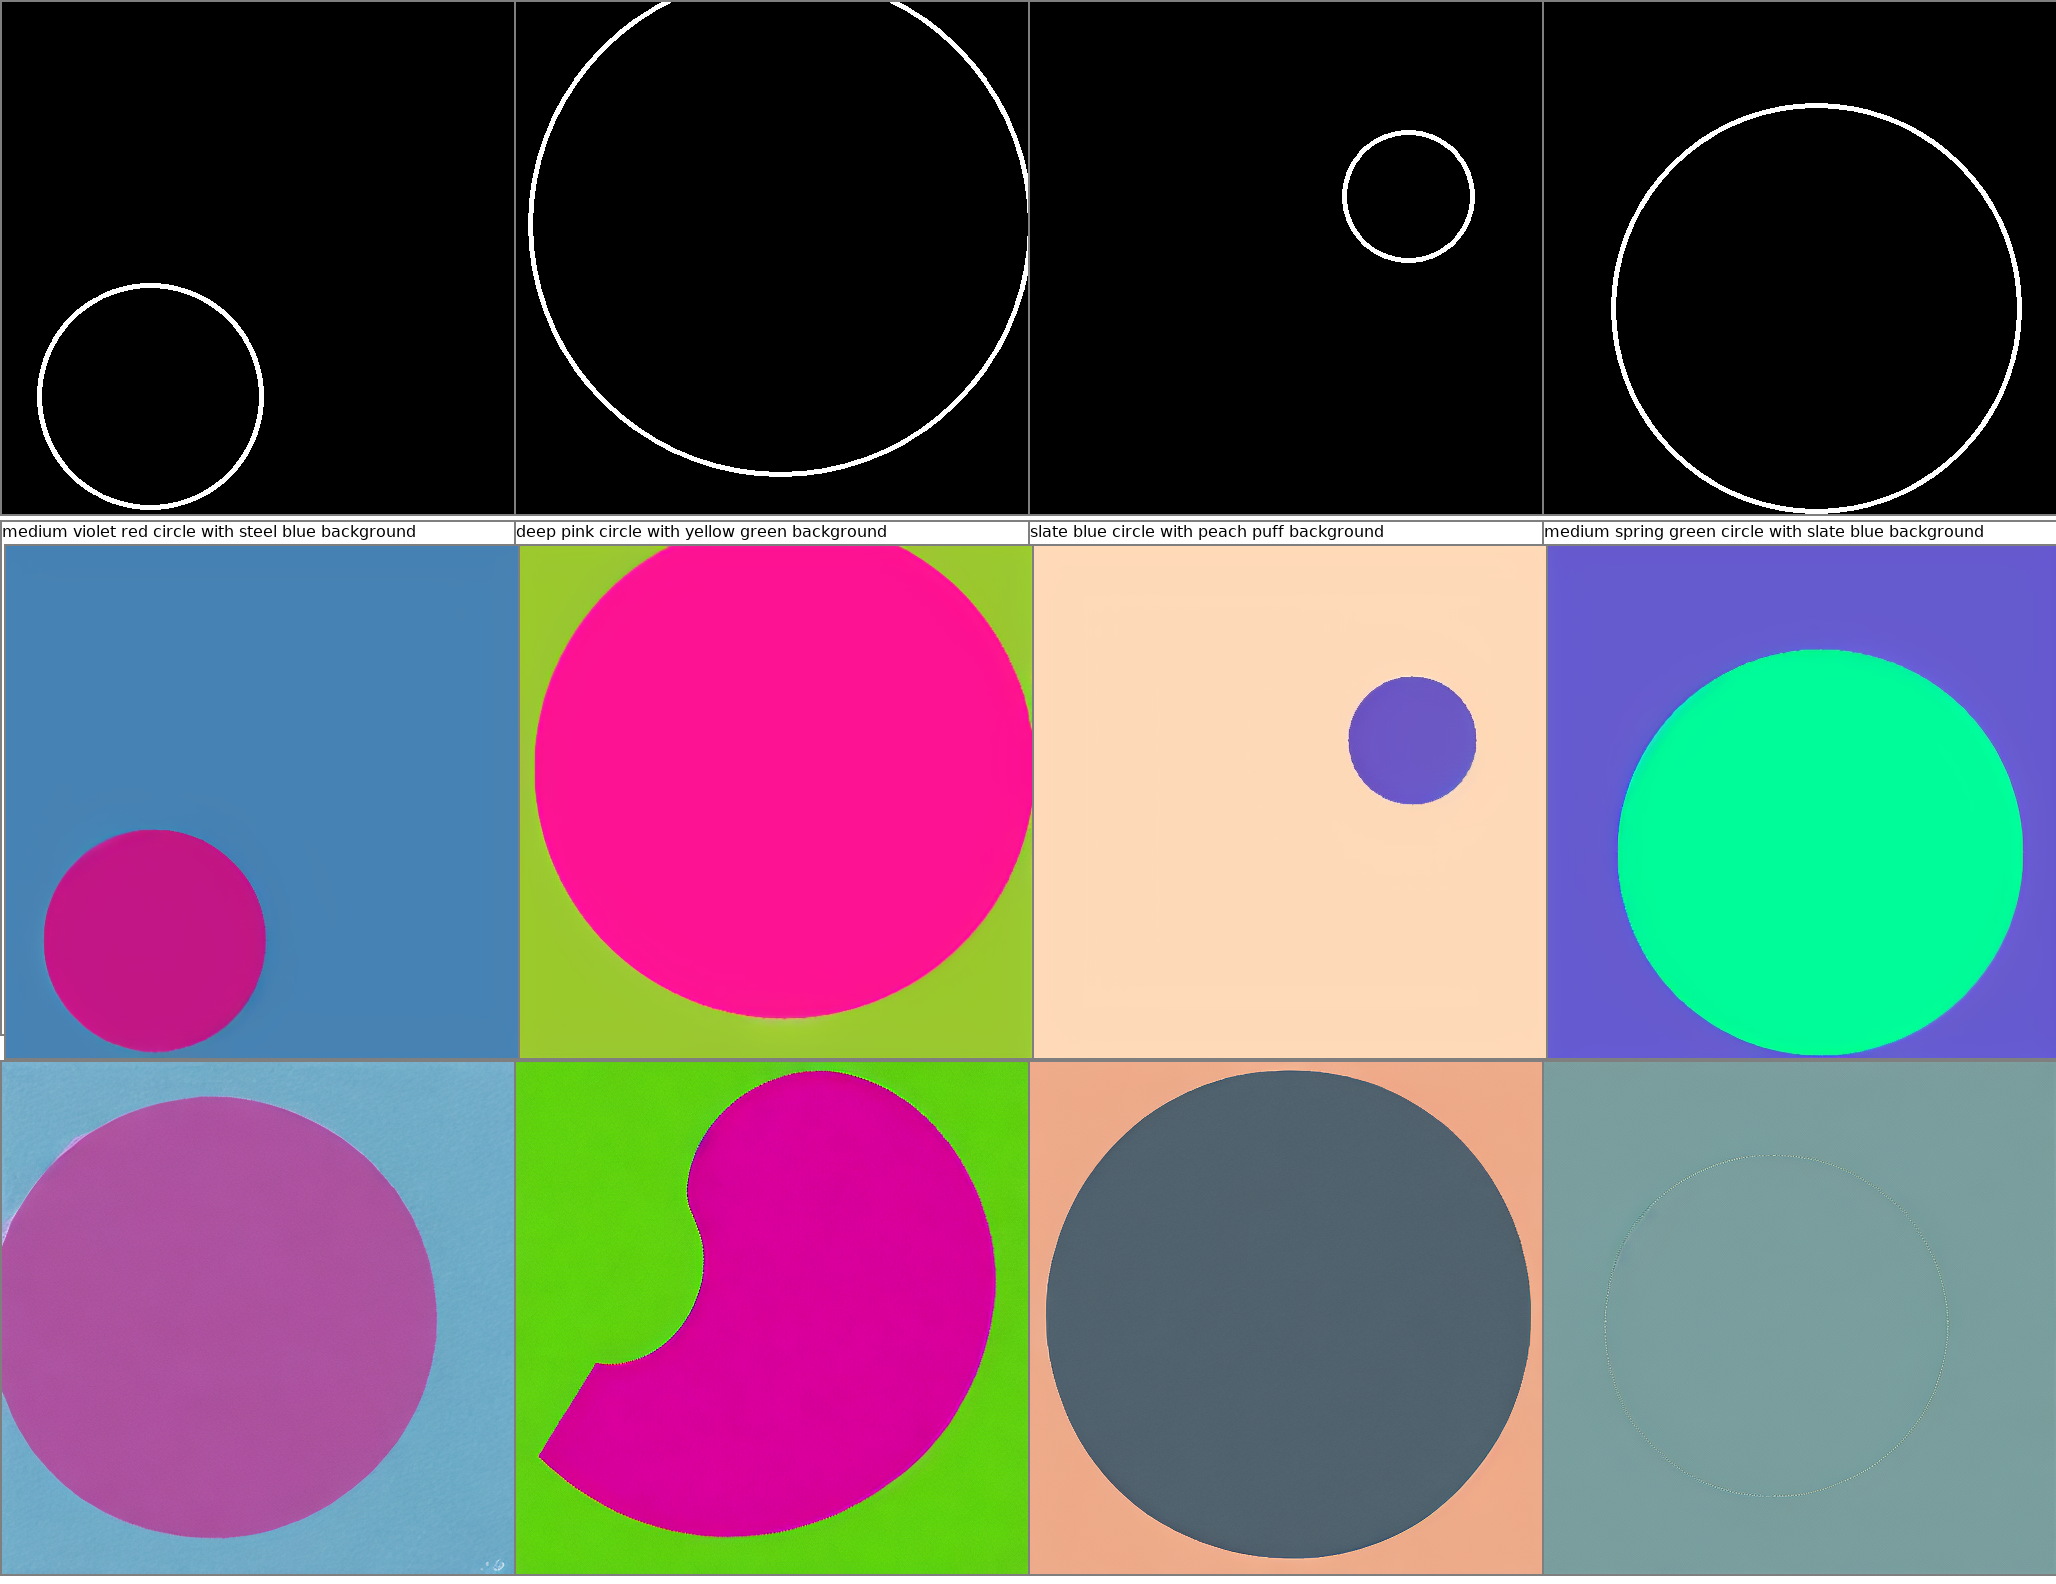
\includegraphics[width=1\linewidth]{t1e0.png}
    \caption{Example1}
\end{figure}

\begin{figure}
    \centering
    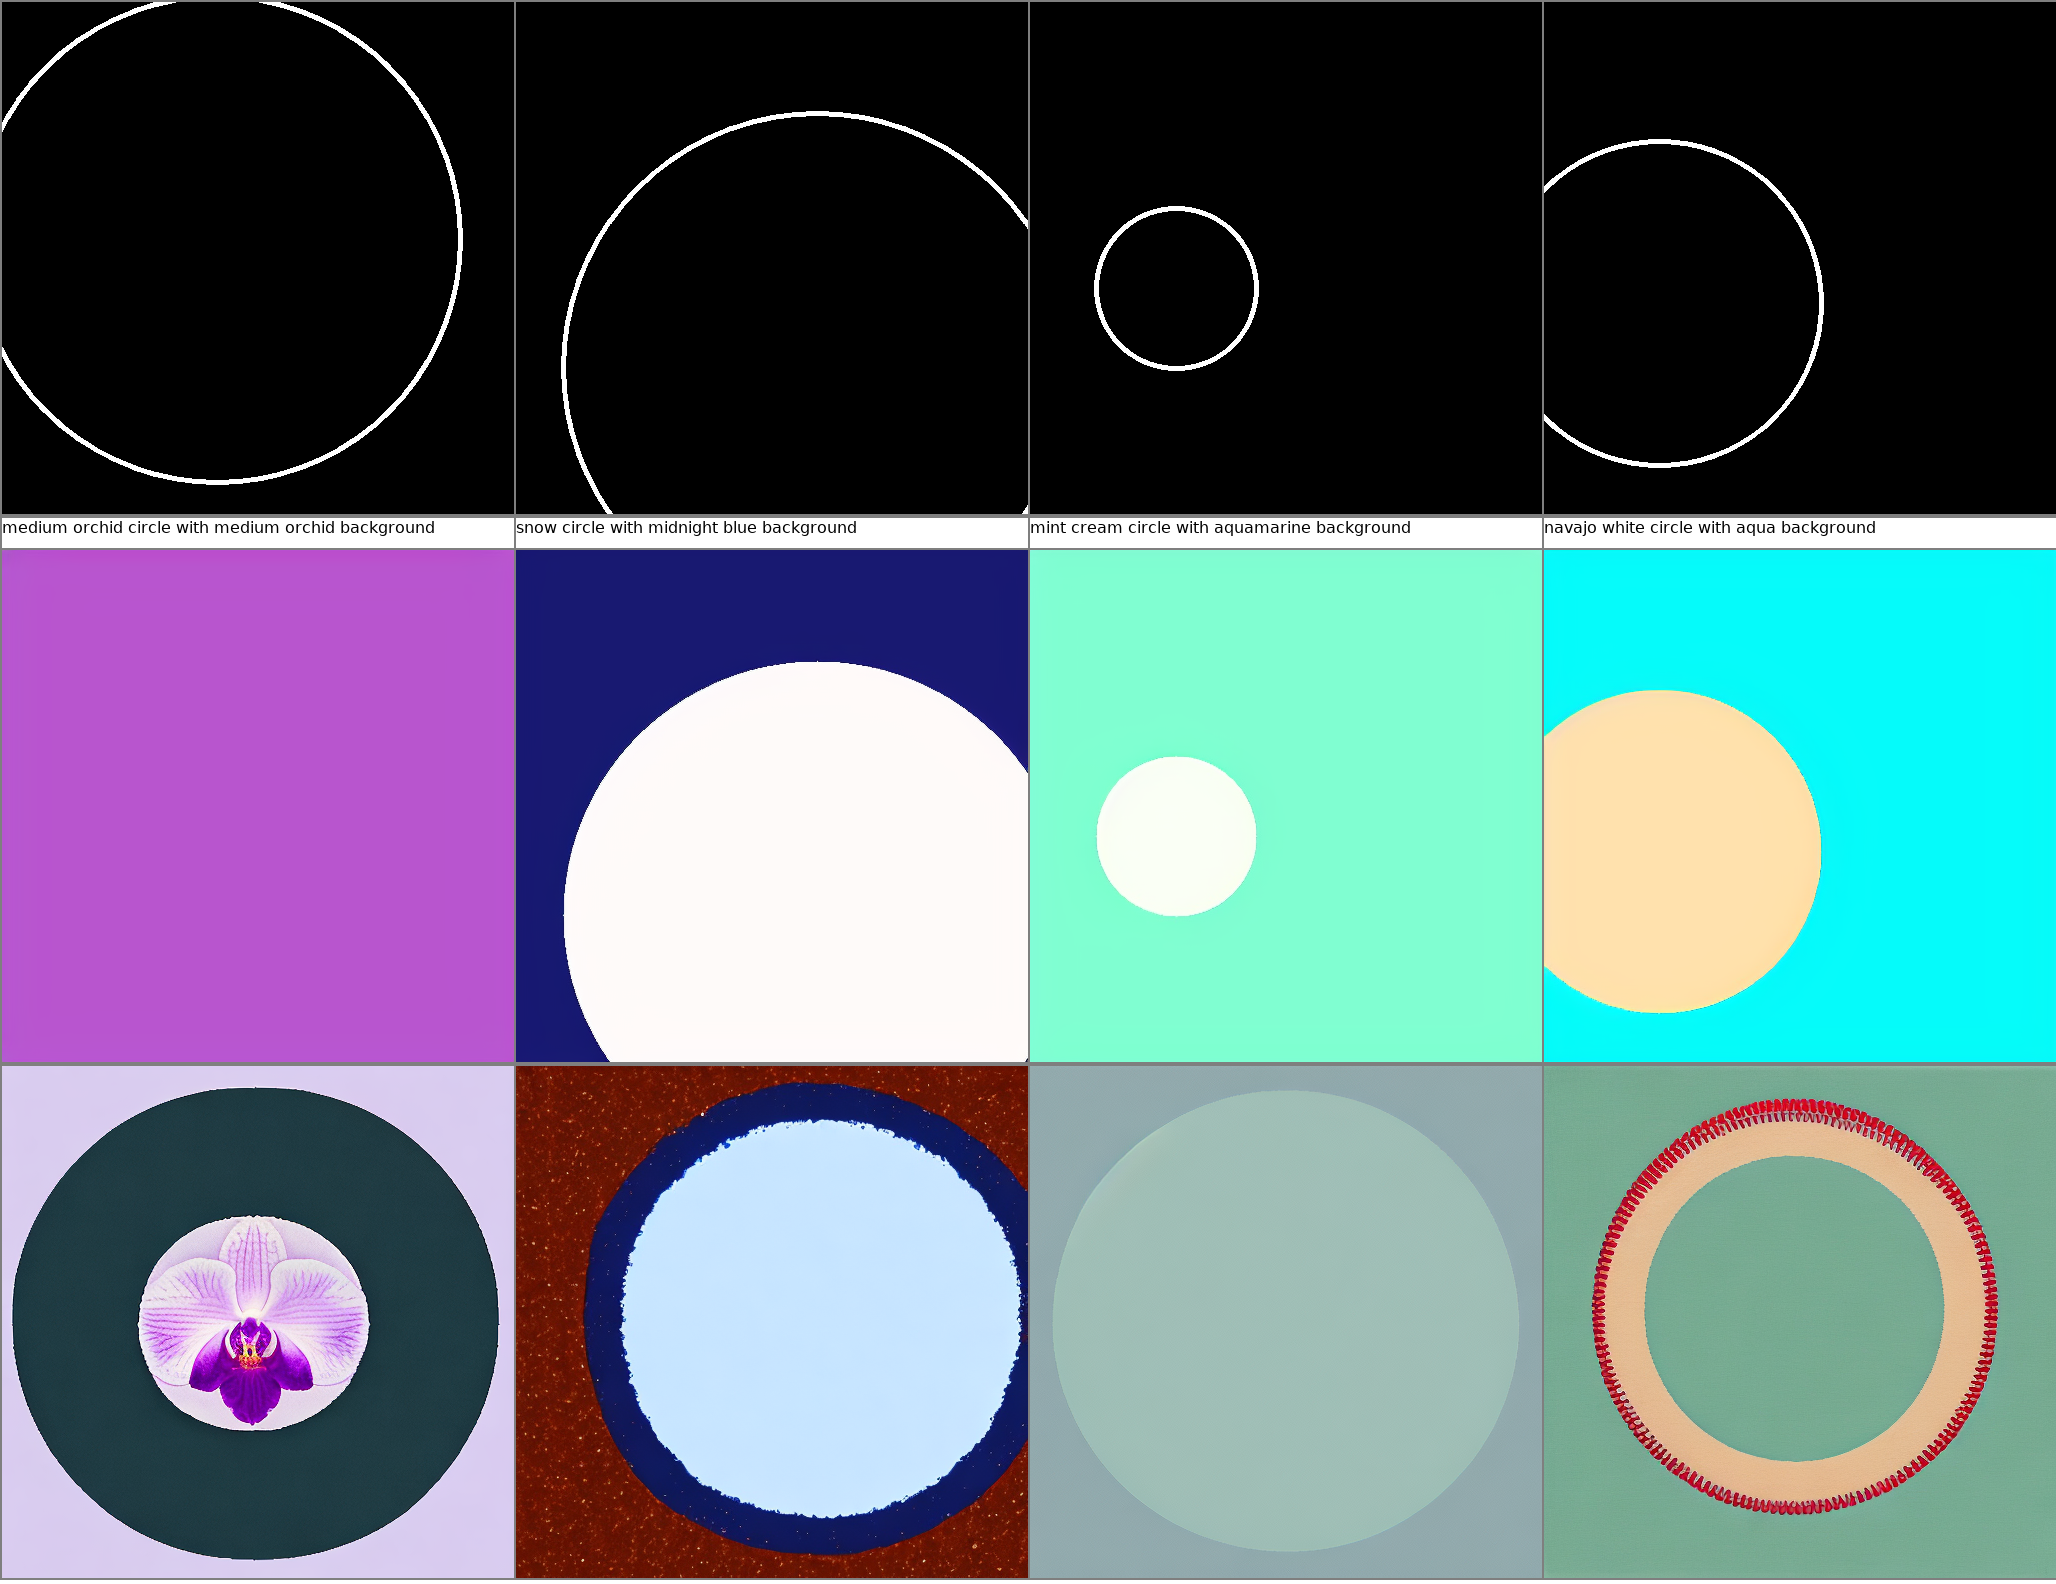
\includegraphics[width=1\linewidth]{t1e2.png}
    \caption{Example2}
\end{figure}



\end{document}
